
          %---------%
\chapter{~~Remeshing}\label{\numb section 10}
          %---------%

This section is devoted to remeshing algorithms.
Before proceeding please make sure you have read and understood paragraphs
\ref{\numb section 9.\numb parag 6} and \ref{\numb section 9.\numb parag 7}.


          %---------------------------------%
\section{~~Cutting a square along a diagonal}\label{\numb section 10.\numb parag 1}
          %---------------------------------%

Suppose we have a mesh of squares and for some reason we want to transform one of the
squares in two triangles, cutting it along one of its diagonals.

One way to achieve this is

\begin{Verbatim}[commandchars=\\\{\},formatcom=\small\tt,frame=single,
   label=parag-\ref{\numb section 10.\numb parag 1}.cpp,rulecolor=\color{coment},
   baselinestretch=0.94,framesep=2mm]
   ABCD .remove_from_mesh ( msh );
   \verm{Cell} \azul{AC} ( \textcolor{tag}{tag}::segment, A .reverse(), C );
   \verm{Cell} \azul{ABC} ( \textcolor{tag}{tag}::triangle, AB, BC, AC .reverse() );
   \verm{Cell} \azul{CDA} ( \textcolor{tag}{tag}::triangle, CD, DA, AC );
   ABC .add_to_mesh ( msh );
   CDA .add_to_mesh ( msh );
\end{Verbatim}

\begin{figure}[ht] \centering
  \psfrag{A}{\small\tt\textcolor{textindraw}{A}}
  \psfrag{B}{\small\tt\textcolor{textindraw}{B}}
  \psfrag{C}{\small\tt\textcolor{textindraw}{C}}
  \psfrag{D}{\small\tt\textcolor{textindraw}{D}}
  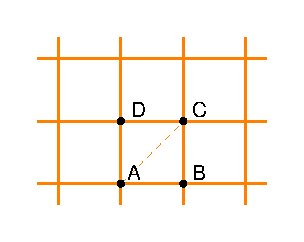
\includegraphics[width=60mm]{malha-quadr}
  \caption{A (part of a) mesh of squares}
  \label{\numb section 10.\numb fig 1}
\end{figure}

The only delicate point here is that the core of the {\small\tt\verm{Cell}} object
{\small\tt ABCD}
will become unused (and inaccessible when the wrapper goes out of syntactic scope).
If you have the garbage collector on (see paragraph \ref{\numb section 11.\numb parag 5}),
the core will be destroyed when the wrapper goes out of scope.
Otherwise, the core will continue to occupy space in the computer's memory giving rise
to an undesirable phenomenon known as ``memory leak''.
If your program does this a lot, it will occupy increasingly more memory without reason.


           %-------------------------------------%
\section{~~{Transforming a square into a triangle}}\label{\numb section 10.\numb parag 2}
           %-------------------------------------%

Instead of discarding the square and building two new triangles, we can use the same
{\small\tt\verm{Cell}} object {\small\tt ABCD}
by transforming it into a triangle, without removing it from {\small\tt msh}, then add
a new triangle to obtain the same result as in paragraph \ref{\numb section 10.\numb parag 1}.

\begin{Verbatim}[commandchars=\\\{\},formatcom=\small\tt,frame=single,
   label=parag-\ref{\numb section 10.\numb parag 2}.cpp,rulecolor=\color{coment},
   baselinestretch=0.94,framesep=2mm]
   CD .cut_from_bdry_of ( ABCD );
   DA .cut_from_bdry_of ( ABCD );
   \cinza{// at this point, ABCD is a cell whose boundary is incomplete}
   \cinza{// it has only two sides and an opening}
   \cinza{// however, it still is part of 'msh'}

   \verm{Cell} \azul{AC} ( \textcolor{tag}{tag}::segment, A .reverse(), C );
   AC .reverse() .glue_on_bdry_of ( ABCD );
   \cinza{// at this point, and in spite of its name, ABCD is no longer a square}
   \cinza{// it is a triangle, still part of 'msh'}

   \verm{Cell} \azul{CDA} ( \textcolor{tag}{tag}::triangle, CD, DA, AC );
   CDA .add_to_mesh ( msh );
\end{Verbatim}



          %--------------------------------%
\section{~~Modifying the mesh within a loop}\label{\numb section 10.\numb parag 3}
          %--------------------------------%

As is the case with many {\tt C++} containers, it is not safe to modify a mesh while
iterating over its cells.
For instance, code below gives undefined behaviour (often, a {\small\tt segmentation fault}
will occur).

\begin{Verbatim}[commandchars=\\\{\},formatcom=\small\tt,frame=single,
   label=incorrect code !,rulecolor=\color{coment},
   baselinestretch=0.94,framesep=2mm]
   \verm{CellIterator} \azul{it} = msh .iterator ( \textcolor{tag}{tag}::over_cells_of_dim, 2 );
   for ( it .reset(); it .in_range(); it++ )
   \{  \verm{Cell} \azul{square} = *it;
      if ( \cinza{... some criterion ...} )
      \{  square .remove_from_mesh ( msh );
         \cinza{// statement above opens the path to disaster}
         \cinza{// next time 'it' is incremented, we get undefined behaviour}
         \cinza{// we may add other cells afterwards, at no good}
         some_other_cell .add_to_mesh ( msh );     \}   \}
\end{Verbatim}

We can circumvent this problem by creating a list of cells to be cut.

\begin{Verbatim}[commandchars=\\\{\},formatcom=\small\tt,frame=single,
   label=parag-\ref{\numb section 10.\numb parag 3}.cpp,rulecolor=\color{coment},
   baselinestretch=0.94,framesep=2mm]
   std::list < \verm{Cell} > list_of_squares;

   \verm{CellIterator} \azul{it} = msh .iterator ( \textcolor{tag}{tag}::over_cells_of_dim, 2 );
   for ( it .reset(); it .in_range(); it++ )
   \{  \verm{Cell} \azul{square} = *it;
      if ( \cinza{ \mbox{\fontfamily{helvetica}\selectfont{}some criterion} } )  \cinza{// we decide to cut this square in halves}
         list_of_squares .push_back ( square );  \}

   for ( std::list < \verm{Cell} > ::iterator \azul{it_square} = list_of_squares .begin(),
         it_square != list_of_squares .end(); it_square               )
   \{  \verm{Cell} \azul{square} = * it_square;
      \cinza{// according to the same criterion, choose a diagonal, here we cut along PR}
      square .remove_from_mesh ( msh );
      \verm{Cell} \azul{PR} ( \textcolor{tag}{tag}::segment, P .reverse(), R );
      \verm{Cell} \azul{PQR} ( \textcolor{tag}{tag}::triangle, PQ, QR, PR .reverse() );
      PQR .add_to_mesh ( msh );
      \verm{Cell} \azul{RSP} ( \textcolor{tag}{tag}::triangle, RS, SP, PR );
      RSP .add_to_mesh ( msh );                           \}
\end{Verbatim}


          %-----------------------------%
\section{~~Improving a mesh of triangles}\label{\numb section 10.\numb parag 4}
          %-----------------------------%

Sometimes the progressive meshing algorithm, presented in section \ref{\numb section 3},
produces imperfect meshes.
Recall that this algorithm produces meshes of triangles.
For such a mesh to be considered of good quality, one may require each inner vertex
to have six neighbour triangles, and thus six neighbour segments.
This is not realistic for arbitrary domains, but it is reasonable to require each vertex
to have five, six or seven neighbours.
In most cases, the algorithm fulfills this condition, but in rare cases we can see vertices
with four or eight vertices (in extremely rare cases vertices with three neighbours show up).

The code presented in this section searches for vertices with four (or three) neighbours,
as well as vertices with eight (or more) neighbours.
It then performs a ``flip'' operation in order to fix this undesired configuration.
Figure \ref{\numb section 10.\numb fig 2} illustrates this operation.
On the right hand side, we see that the red vertex has only four neighbours.
After ``flipping'' the blue segment, the red vertex will have five neighbours.

\begin{figure}[ht] \centering
  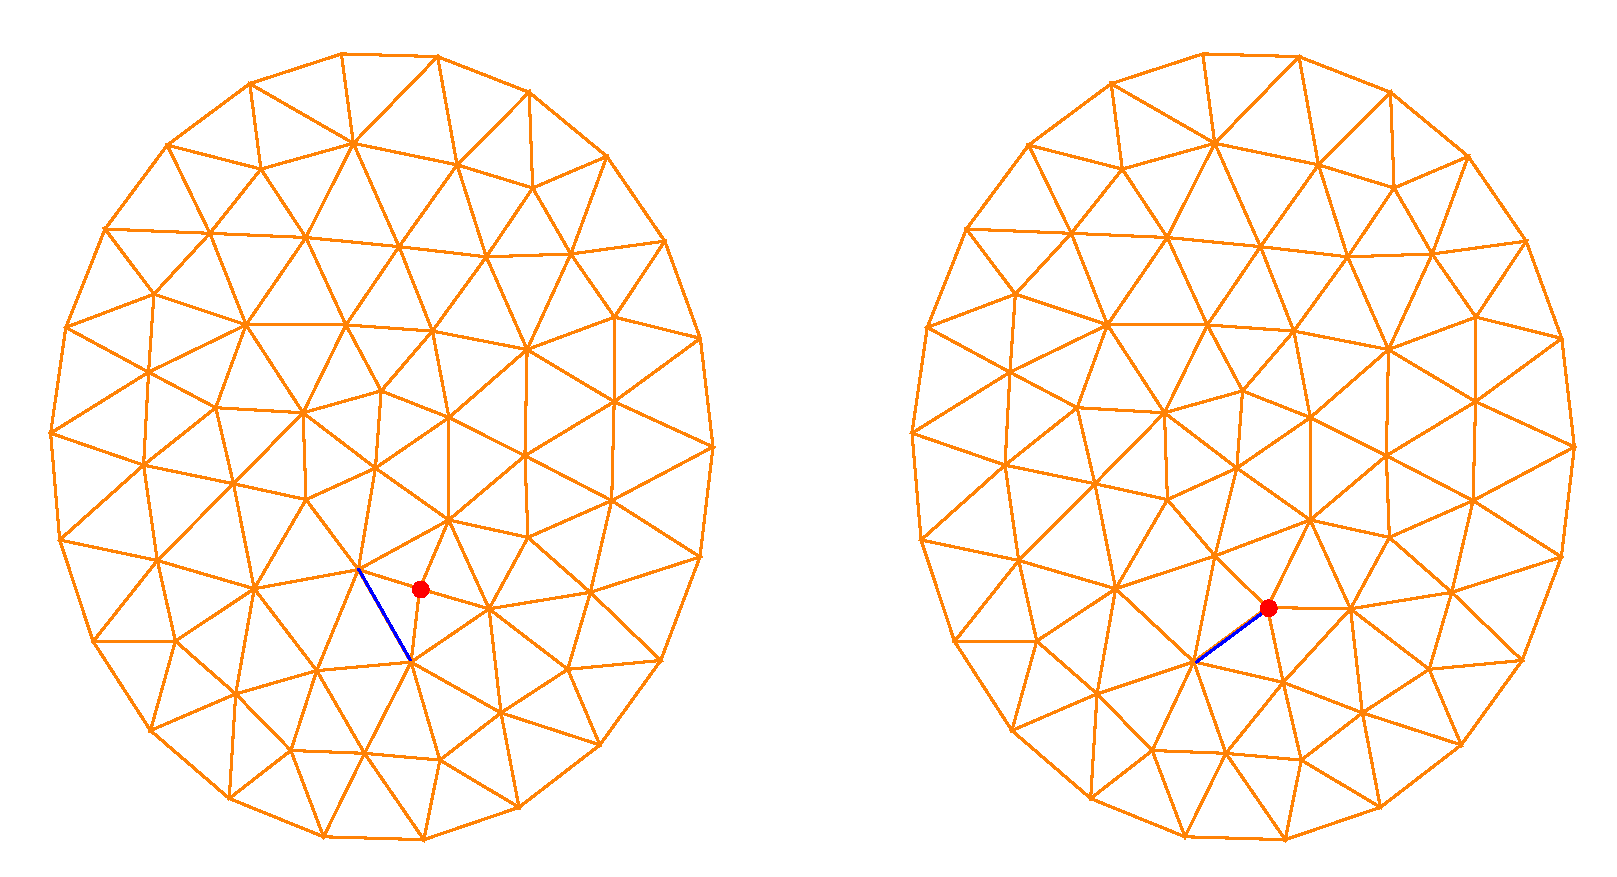
\includegraphics[width=127mm]{two-ellipses}
  \caption{Left : before remeshing, right : after remeshing}
  \label{\numb section 10.\numb fig 2}
\end{figure}

Below is the code performing the ``flip'' operation.

\begin{Verbatim}[commandchars=\\\{\},formatcom=\small\tt,frame=single,
   label=parag-\ref{\numb section 10.\numb parag 3}.cpp,rulecolor=\color{coment},
   baselinestretch=0.94,framesep=2mm]
inline bool \azul{flip_segment} ( \verm{Mesh} & \azul{msh}, \verm{Cell} & \azul{seg} )

\cinza{// flip 'seg' if it is inner to 'msh'}
\cinza{// equilibrates (baricenter) the four neighbour vertices}

\cinza{// return true if the segment has been flipped, false if not}

\cinza{// assumes there are only triangular cells}
	
\cinza{// assumes there is no higher-dimensional mesh "above" 'msh'}

\{  \verm{Cell} \azul{tri2} = msh .cell_in_front_of ( seg, \textcolor{tag}{tag}::may_not_exist );
   if ( not tri2.exists() ) return false; 
   \verm{Cell} \azul{tri1} = msh .cell_behind ( seg, \textcolor{tag}{tag}::may_not_exist );
   if ( not tri1 .exists() ) return false;
   \cinza{// or, equivalently :  if ( not seg .is_inner_to ( msh ) ) return false}

   \verm{Cell} \azul{A} = seg .base() .reverse();
   \verm{Cell} \azul{B} = seg .tip();
   \verm{Cell} \azul{BC} = tri1 .boundary() .cell_in_front_of ( B, \textcolor{tag}{tag}::surely_exists );
   \verm{Cell} \azul{CA} = tri1 .boundary() .cell_behind ( A, \textcolor{tag}{tag}::surely_exists );
   \verm{Cell} \azul{AD} = tri2 .boundary() .cell_in_front_of ( A, \textcolor{tag}{tag}::surely_exists );
   \verm{Cell} \azul{DB} = tri2 .boundary() .cell_behind ( B, \textcolor{tag}{tag}::surely_exists );
   \verm{Cell} \azul{C} = BC .tip();
   assert ( CA .base() .reverse() == C );
   \verm{Cell} \azul{D} = AD.tip();
   assert ( DB .base() .reverse() == D );
	
   B .cut_from_bdry_of ( seg, \textcolor{tag}{tag}::do_not_bother );
   A .reverse() .cut_from_bdry_of ( seg, \textcolor{tag}{tag}::do_not_bother );
   \cinza{// at this point, 'seg' is a weird segment with no extremities at all}
     
   CA .cut_from_bdry_of ( tri1, \textcolor{tag}{tag}::do_not_bother );
   DB .cut_from_bdry_of ( tri2, \textcolor{tag}{tag}::do_not_bother );
   \cinza{// 'tri1' and 'tri2' now have as boundaries open chains of two segments only}
   \cinza{// even worse : one of these segments is 'seg' which is itself incomplete}
   \cinza{//              so these chains are actually disconnected}
   
   C .reverse() .glue_on_bdry_of ( seg, \textcolor{tag}{tag}::do_not_bother );
   D .glue_on_bdry_of ( seg, \textcolor{tag}{tag}::do_not_bother );
   \cinza{// 'seg' is complete again}
   \cinza{// boundaries of 'tri1' and 'tri2' are now connected chains of two segments each}
   
   DB .glue_on_bdry_of ( tri1, \textcolor{tag}{tag}::do_not_bother );
   CA .glue_on_bdry_of ( tri2, \textcolor{tag}{tag}::do_not_bother );
   \cinza{// 'tri1' and 'tri2' are complete again, their boundaries are closed loops}

   tri1 .boundary() .closed_loop ( B );
   tri2 .boundary() .closed_loop ( A );

   if ( A .is_inner_to ( msh ) ) msh .baricenter ( A );
   if ( B .is_inner_to ( msh ) ) msh .baricenter ( B );
   if ( C .is_inner_to ( msh ) ) msh .baricenter ( C );
   if ( D .is_inner_to ( msh ) ) msh .baricenter ( D );

   return true;

\}  \cinza{// end of  flip_segment}
\end{Verbatim}

Code above follows the approach, already used in paragraph \ref{\numb section 10.\numb parag 2},
of destroying partially cells (segments and triangles) and then completing them later
in a different configuration.
In contrast, paragraphs \ref{\numb section 10.\numb parag 1} and
\ref{\numb section 10.\numb parag 3} show code which simply removes cells from the mesh
then builds entirely new cells and adds them to the mesh.

In the above code, we add a {\small\tt\textcolor{tag}{tag}::do\_\,not\_\,bother} as argument
to methods {\small\tt cut\_\,from\_\,bdry\_\,of} and {\small\tt glue\_\,on\_\,bdry\_\,of}.
This tag changes the behaviour of the respective methods when a
{\small\tt\verm{Mesh}::Connected::OneDim} is involved
(paragraph \ref{\numb section 11.\numb parag 6} gives details on different kinds of meshes).
Recall that boundaries of triangles (and of other two-dimensional cells) are
{\small\tt\verm{Mesh}::Connected:: ::OneDim} if built through the usual constructors.

Methods {\small\tt cut\_\,from\_\,bdry\_\,of} and {\small\tt glue\_\,on\_\,bdry\_\,of},
if invoked without the {\small\tt\textcolor{tag}{tag}::do\_\,not\_\,bother},
when trying to add or remove cells from a {\small\tt\verm{Mesh}::Connected::OneDim},
take care to leave that mesh in a consistent state.
Removing a cell from a closed loop transforms it into an open chain of segments;
the reverse may happen when adding a cell.
Also, the number of component segments must be kept up-to-date.

If we provide the {\small\tt\textcolor{tag}{tag}::do\_\,not\_\,bother} to these methods,
they will not waste computing time with such details.
The respective meshes will be left in an inconsistent state.
That's why we use the method {\small\tt closed\_\,loop} and provide a vertex;
this method fixes the state of the mesh.
We could also provide the updated number of segments as second argument to method
{\small\tt closed\_\,loop}; this is not necessary in this case because the number of
segments has not changed.
